\subsection{Überarbeitung der Vergleichsalgorithmen}

Das ausschlaggebende Feature der Software ist ihre Ähnlichkeitsmatrix. Diese wurde bereits in der Einleitung kurz erwähnt. Auch die Funktionsweisen der beiden Vergleichsalgorithmen \textit{Line Compare} und \textit{Character Compare} wurden bereits oberflächlich behandelt. Dieses Unterkapitel behandelt nun die Überarbeitung des Modus Line Compare und die Einführung zweier neuer Vergleichsmodi, die sich in ihrer Funktionsweise stark von den bisherigen Algorithmen unterscheiden.

\subsubsection{Zeilenweiser Vergleich regulärer Textdateien}

Line Compare war der erste Vergleichsmodus der Software. Da zum Zeitpunkt der Entwicklung noch keine Matching-Komponente existierte, arbeitete der Vergleichsmodus nicht mehr optimal sobald ähnliche Zeilen leicht verschoben waren. Das Ziel ist nun die Einbettung der Matching-Komponente in den regulären Textvergleich um Dateien, die dem Benutzer in der Diff-Anzeige als ähnlich angezeigt werden würden, auch mit einer höheren Genauigkeit für den Vergleich bewerten zu können.

Alle Vergleiche basieren auf den von der Komponente \emph{FileImporter} erstellten temporären Dateien. Diese sind notwendig um die vom Benutzer ausgewählten Originaldateien bei einer Normierung, also zum Beispiel einer Entfernung aller Leerzeichen, nicht zu verändern. Des Weiteren wurde explizit für den Line Compare Modus ein weiteres Set an temporären Dateien erstellt, bei denen nach jedem Wort ein Zeilenumbruch eingefügt wurde. Als Wort galt eine beliebige Zeichenkette gefolgt von einem Leerzeichen.  

Dieser Prozess sollte eigentlich dazu dienen, um die Genauigkeit des Vergleichs leicht zu verbessern, wobei dies nur für Dateien funktioniert, die ohnehin ähnliche Zeileneinträge in der gleichen Reihenfolge besitzen.

Um die Matching-Komponente in den Vergleich einzubinden, muss zunächst ihre Schnittstelle angepasst werden. Aktuell hat die Matching-Methode \textit{matchLines()} nämlich noch den Rückgabetyp void, denn ihre Erzeugnisse waren bisher immer neue temporäre Dateien im Dateisystem auf die andere Komponenten zugreifen konnten. Um IO-Zugriffe zwecks Laufzeit zu minimieren, erstellt die Methode diese temporären Dateien nicht falls sie für den Vergleich aufgerufen wird. Stattdessen werden die gematchten Zeilen als ein \textit{Object}-Array zurückgegeben. So kann der Rest des Vergleichsalgorithmus unverändert bleiben. Das heißt, dass Zeilen des gleichen Index nach dem in Abschnitt \ref{Levenshtein-Distanz} beschriebenen Verfahren bewertet werden. Sind die beiden zu vergleichenden Dateien nicht gleich lang, wird die kürzere Datei mit Leerzeilen aufgefüllt. Das Ergebnis ist ein zeilenbasierter Vergleichsalgorithmus, der nun verschobene Zeilen erkennen und genauer bewerten kann. Gleichzeitig profitiert er von den in Kapitel \ref{verbesserungMatching} durchgeführen Verbesserungen.

\subsubsection{Vergleich von XML-Dateien}\label{xmlChapter}

\paragraph{Erweiterung der Element-Sortierung}\mbox{}\label{xmlSortierung}

In Version 1.0 besteht bereits die Möglichkeit, die Strukturbäume von XML-Dateien nach ihren Element-Namen und Attribut-Namen zu sortieren. Die Sortierung der Attribute ist insofern eindeutig, als dass ein Attributname pro Element immer einzigartig sein muss. Für Elemente gibt es allerdings keine solche Regel. Elemente, die den gleichen Namen haben und auf der gleichen Ebene innerhalb des Baumgraphen liegen, können als Liste interpretiert werden. 

Vergleichsoperationen wie Line Compare und die Berechnung der Diff würden davon profitieren, wenn XML-Dateien eindeutig sortiert werden könnten, da sie zeilenbasiert operieren. Wenn ähnliche Zeilen in der gleichen Reihenfolge vorliegen, können sie zusätzlich durch das Zeilenmatching erkannt werden. Da weder durch die XML-Spezifikation noch durch die JDOM-API eine Sortierreihenfolge vorgeschrieben wird, wird im Folgenden eine eigene Reihenfolge festgelegt. Diese Priorisierung bezieht sich auf den Vergleich von zwei Elementen:

\newpage
\begin{enumerate}
    \item Elementname
    \item Attributname
    \item Attributwert
    \item Textinhalt
\end{enumerate}

Die Implementierung erfolgt über die Schnittstelle \emph{java.util.Comparator} und das Überschreiben ihrer \textit{compare()}-Methode. Diese gibt einen Integer-Wert zurück mit Hilfe dessen zwei Strings lexikographisch als kleiner, größer oder gleich bewertet werden können. Diese Bewertung wird durch die von JDOM breitgestellte Methode \textit{sortChildren()} ausgewertet, um die Elemente strukturerhaltend zu sortieren.

Sind die Elementnamen identisch, werden die Attribute untersucht. Da Elemente beliebig viele Attribute haben können, werden zunächst nur so viele Attribute verglichen, wie in der kürzesten Attributliste vorhanden sind. Dabei werden erst die Attributnamen verglichen und dann die Werte. Dafür ist vorausgesetzt, dass die Attribute vorher bereits sortiert wurden. Sind die bisher betrachteten Attribute sowohl im Namen als auch im Wert identisch, entscheidet die Anzahl der Attribute. Mehr Attribute werden dabei als größer eingestuft. Bei gleicher Attributzahl werden letztlich noch die Textknoten der Elemente miteinander verglichen. Falls alle dieser Kriterien für die beiden Elemente identisch sind, wird das Verfahren in gleicher Reihenfolge rekursiv für alle Kindknoten der beiden infrage stehenden Elemente durchgeführt, bis ein Unterschied festgestellt wird. Bei Gleichheit der Elemente wird nichts verändert.

\paragraph{Struktureller Vergleich von XML-Dateien}\mbox{}

Im Vorfeld wurden bereits Limitationen der vorhandenen Vergleichsalgorithmen diskutiert. Weder der zeilen- noch der zeichenbasierte Vergleichsansatz kann für Dateien, die einer gewissen Struktur unterliegen zuverlässig für akkurate Ergebnisse sorgen. Aus diesem Grund wird im Folgenden ein Vergleichsalgorithmus entworfen und implementiert, der XML-Dateien auf Basis der Baumstruktur vergleicht.

Verglichen werden sollen dabei die Element-, Attribut-, Text-, CDATA- und Kommentarknoten, wobei letztere optional sind und durch einen Konfigurationsparameter vom Vergleich ausgeschlossen werden können. Ausschlaggebend für den Vergleich sind allerdings die Elementknoten, da jeder der zuvor genannten Knotentypen ein zugehöriges Elternelement hat. Die einzige Ausnahme ist der Wurzelknoten, wobei dieser vom Vergleich ausgenommen ist. Um \emph{false positives} zu vermeiden werden zwei Elemente nur miteinander verglichen werden, wenn ihre Namen identisch sind.

Durch diesen verschiedenen Ansatz, kann das alte Bewertungssystem für die Ähnlichkeit über die LCS oder die Levenshtein-Distanz hier nicht verwendet werden. Stattdessen wird für den strukturellen Vergleich ein Ähnlichkeitsmaß auf Basis der Baumstruktur eingeführt. In Abb. \ref{fig:ähnlichkeitBaum} ist ein Beispielbaum dargestellt, für den die Gewichte der Knoten an der Kante zum Elternelement annotiert sind. Für eine sinnvolle Bewertung wird hierbei davon ausgegangen, dass innerhalb der zu vergleichenden XML-Dateien wichtige Informationen nah am Wurzelelement liegen. Zunächst wird geschaut, wieviele Elemente $n$ innerhalb der ersten Ebene liegen. Jedes dieser Elemente geht mit einem Gewicht von \( \frac{1}{n} \) in den Gesamtwert der Ähnlichkeit ein. Gleichzeitig wirkt dieses Gewicht als ein Budget für dessen Kindelemente. Im Beispiel hat Knoten 2 ein Gewicht von \( \frac{1}{3} \), welches gleichmäßig auf die Kindknoten verteilt wird. Die beiden Kindknoten 5 und 6 haben also im Kontext von Knoten 2 ein Gewicht von \( \frac{1}{2} \). Das Gewicht eines Knotens für die Gesamtähnlichkeit wird berechnet aus dem Produkt aller Kantengewichte $f(V_1,V_2)$ auf dem Weg zwischen der Wurzel und genau diesem Knoten. Dadurch ergibt sich für Knoten 5 bspw. ein Gesamtgewicht von
\[ f(1,2) \cdot f(2,5) = \frac{1}{3} \cdot \frac{1}{2} = \frac{1}{6}\]
\begin{figure}
    \centering
    
\tikzset{eln/.style={midway, font = \Large,inner sep=2pt, outer sep=.30cm}}
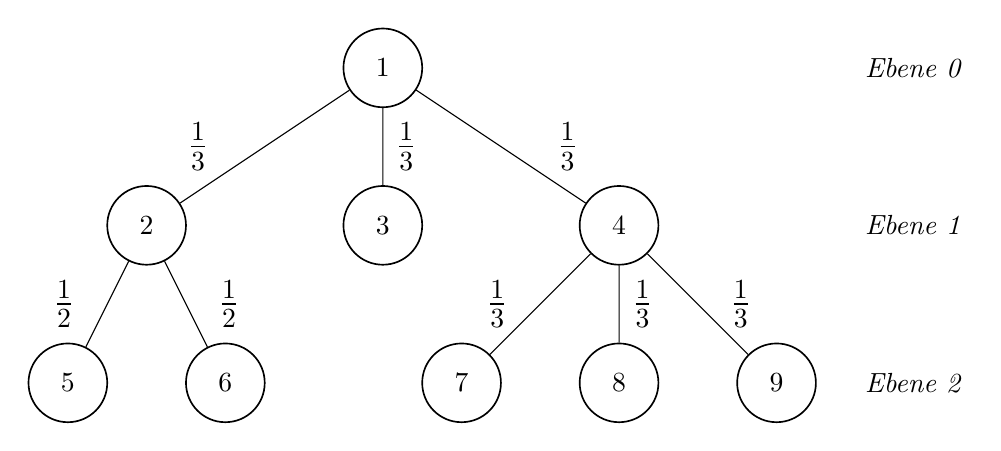
\begin{tikzpicture}[level distance=2cm,
  level 1/.style={sibling distance=3cm},
  level 2/.style={sibling distance=2cm},
  element/.style={circle, draw=black, fill=white, semithick, minimum size=10mm, align=center},
  attribute/.style={ draw=red, fill=white, semithick, minimum size=7mm, align=center},
  textnode/.style={ draw=black, fill=white, semithick, minimum size=7mm, align=center}]
  \node [element](Root){1}
    child {node [element]{2} 
      child {node [element]{5} edge from parent node[left,font = \Large, outer sep=.30cm]{ \( \frac{1}{2} \)} }
      child {node [element]{6} edge from parent node[right,font = \Large, outer sep=.30cm]{ \( \frac{1}{2} \)} }
      edge from parent node[left,font = \Large, outer sep=.60cm]{ \( \frac{1}{3} \)}
    }
    child {node [element]{3} edge from parent node[right,font = \Large, outer sep=0.5mm]{ \( \frac{1}{3} \)}}
    child {node [element]{4}
      child {node [element]{7} edge from parent node[left,font = \Large, outer sep=.30cm]{ \( \frac{1}{3} \)}}
      child {node [element]{8} edge from parent node[right,font = \Large, outer sep=0.5mm]{ \( \frac{1}{3} \)}}
      child {node [element]{9} edge from parent node[right,font = \Large, outer sep=.30cm]{ \( \frac{1}{3} \)}}
      edge from parent node[right,font = \Large, outer sep=.60cm]{ \( \frac{1}{3} \)}
    };
    \begin{scope}[every node/.style={right}]
     \path (Root    -| Root-3-3) ++(5mm,0) node{}  ++(5mm,0) node {\emph{Ebene 0}};
     \path (Root-1  -| Root-3-3) ++(5mm,0) node{}  ++(5mm,0) node{ \emph{Ebene 1}};
     \path (Root-1-1-| Root-3-3) ++(5mm,0) node{}  ++(5mm,0) node {\emph{Ebene 2}};
   \end{scope}
\end{tikzpicture}
    \caption{Gewichtung von Elementknoten für strukturellen Vergleich}
    \label{fig:ähnlichkeitBaum}
\end{figure}

Um diese Gewichte einzusetzen, muss noch definiert werden wodurch zwei Knoten ähnlich sind. Dafür wird bei den Kindknoten der Elemente zwischen textuellem Inhalt, Attributen und Kommentaren unterschieden. Falls Kommentare ignoriert werden sollen oder keine Kommentare präsent sind, sind einzig der Text und die Attribute zu bewerten. Sollten auch keine Attribute existieren, zählt nur der Textinhalt bzw. sollte kein Textinhalt existieren, zählen nur die Attribute. Der Textinhalt schließt reine Textknoten und CDATA-Knoten ein, da JDOM hier auch keine explizite Unterscheidung macht und sie häufig den gleichen Zweck erfüllen. Falls Elemente keinerlei Kindknoten haben, sind sie identisch. Wie Abb. \ref{fig:elementähnlichkeit} zeigt, wird jeder dieser Knoten, sofern er existiert, gleichwertig gewichtet.

\begin{figure}
    \centering
    
\tikzset{eln/.style={midway, font = \Large,inner sep=2pt, outer sep=.30cm}}
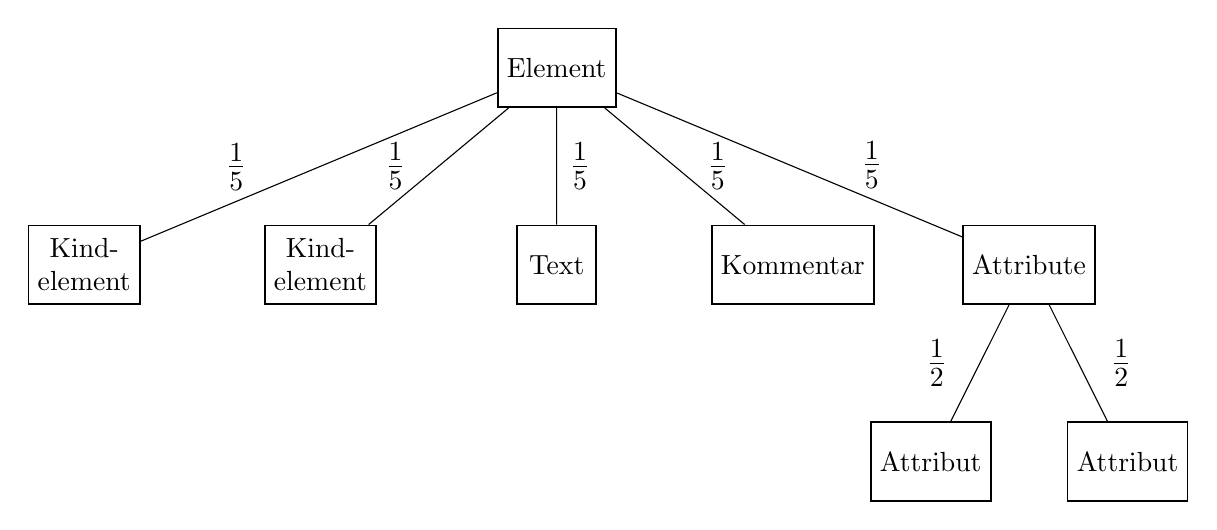
\begin{tikzpicture}[level distance=2.5cm,
  level 1/.style={sibling distance=3cm},
  level 2/.style={sibling distance=2.5cm},
  element/.style={draw=black, fill=white, semithick, minimum size=10mm, align=center},
  attribute/.style={ draw=red, fill=white, semithick, minimum size=7mm, align=center},
  textnode/.style={ draw=black, fill=white, semithick, minimum size=7mm, align=center}]
  \node [element](Root){Element}
    child {node [element]{Kind-\\element}
      edge from parent node[left,font = \Large, outer sep=.80cm]{ \( \frac{1}{5} \)}
    }
    child {node [element]{Kind-\\element}
      edge from parent node[left,font = \Large, outer sep=.30cm]{ \( \frac{1}{5} \)}
    }
    child {node [element]{Text} edge from parent node[right,font = \Large, outer sep=0.5mm]{ \( \frac{1}{5} \)}}
    child {node [element]{Kommentar} edge from parent node[right,font = \Large, outer sep=.30cm]{ \( \frac{1}{5} \)}}
    child {node [element]{Attribute}
      child {node [element]{Attribut} edge from parent node[left,font = \Large, outer sep=.30cm]{ \( \frac{1}{2} \)}}
      child {node [element]{Attribut} edge from parent node[right,font = \Large, outer sep=.30cm]{ \( \frac{1}{2} \)}}
      edge from parent node[right,font = \Large, outer sep=.80cm]{ \( \frac{1}{5} \)}
    };
\end{tikzpicture}
    \caption{Beispielhafte Gewichtung eines Elementinhalts für XML}
    \label{fig:elementähnlichkeit}
\end{figure}

Letztlich muss noch sichergestellt werden, dass das Verfahren symmetrisch ist, also die Reihenfolge der verglichenen Bäume nicht das Ergebnis beeinflusst. Ein Beispiel wäre, wenn der Baum aus Abb. \ref{fig:ähnlichkeitBaum} mit einem Baum verglichen werden würde, der auf Ebene 1 vier Knoten besitzt. In diesem Fall würde die maximale Anzahl an Knoten auf der Ebene entscheidend sein, also läge die maximale Ähnlichkeit der Graphen unabhängig vom Inhalt bei \( \frac{3}{4} \). In jeder Situation bei der unterschiedliche Anzahlen an Einträgen existieren können, wird die gemeinsame Anzahl an gleichen Einträgen durch die maximal verfügbare Anzahl geteilt.  

Implementiert wird dieses Konzept indem zunächst die Wurzelknoten der beiden zu vergleichenden Dateien eingelesen werden, wobei einer der Knoten als Referenzknoten festgelegt wird. Dabei ist nicht wichtig welcher der Knoten die Referenz ist, da in XML das Tauschen von Knoten mit gleichem Elternknoten erlaubt ist. Um diesen Vergleichsmodus anwenden zu können, müssen die jeweiligen XML-Dateien wohlgeformt sein, da ansonsten ein Traversieren der Dokumentbäume nicht möglich ist.

Bei vorliegender Wohlgeformtheit wird zunächst für alle Kindknoten der Referenzwurzel, wie in Quellcode \ref{code:knotenMatching} gezeigt, der aktuelle Knotenname in einer Liste gespeichert. Beim ersten Vorkommen dieses Namens werden alle Elemente mit diesem Namen in einer jeweiligen Liste für Referenzknoten (matchingRef) und Vergleichsknoten (matchingComp) gespeichert. Die Methode \emph{getElementCount()} zählt wie oft ein Elementname in einer Liste vorkommt und sorgt dadurch dafür, dass Elementlisten nicht doppelt eingefügt werden.

\begin{listing}[!h]
\begin{minted}
[
frame=lines,
framesep=2mm,
baselinestretch=1.2,
bgcolor=white,
fontsize=\footnotesize,
linenos
]{java}
        List<Element> matchingRef = new ArrayList<Element>();
        List<Element> matchingComp = new ArrayList<Element>();
        List<Element> refFirstLevelChildren = rootRef.getChildren();
        List<String> refElementNames = new ArrayList<String>();
	for (int i = 0; i < refFirstLevelChildren.size(); i++) {
		Element currentRef = refFirstLevelChildren.get(i);
		String currentRefName = currentRef.getName();
		refElementNames.add(currentRefName);
		if (getElementCount(refElementNames, currentRefName) == 1) {
			matchingRef.addAll(rootRef
					.getChildren(currentRefName));
			matchingComp.addAll(rootComp
					.getChildren(currentRefName));
		}
	}
\end{minted}


\caption{Suche nach gleichnamigen Knoten auf gleicher Ebene}
\label{code:knotenMatching}
\end{listing}\newpage

Da die Matching-Komponente für den strukturellen Vergleich nicht eingesetzt werden kann, muss an dieser Stelle noch ein Mechanismus eingeführt werden um gleiche Listeneinträge zu finden und zu vergleichen. Restliche Listeneinträge können dann noch nach ihrem Index geordnet verglichen werden. Allerdings ist es mit JDOM nicht direkt möglich festzustellen ob zwei Elemente tatsächlich gleich sind ohne alle ihre Kindknoten zu betrachten. Die \emph{equals}()-Methode für die Klasse \emph{Element} prüft nicht auf die inhaltliche Ähnlichkeit sondern ob die Referenz zweier Objekte gleich ist. Dadurch, dass eine rekursive Prüfung aller Kindelemente sehr aufwändig sein kann, wird, wie in Quellcode \ref{code:identischeElemente} gezeigt, mit der Klasse \emph{XMLOutputter} von JDOM gearbeitet. Mit ihr ist es nämlich möglich ein Element als String darzustellen. Da die \emph{equals}()-Methode für Strings \emph{true} zurück gibt sobald die verglichenen Zeichensequenzen identisch sind, kann man auf diese Weise die Gleichheit zweier Objekte feststellen. Um identische Elemente vom rekursiven Vergleich auszuschließen, werden diese durch den Wert \emph{null} ersetzt um sie als bereits bewertet zu kennzeichnen. Nachdem alle verfügbaren Elementknoten miteinander auf Gleichheit untersucht wurden, werden gefundenen null-Werte durch eine Hilfsmethode \emph{clearNullValues}() aus den Listen gestrichen. 

\begin{listing}[!tb]
\begin{minted}
[
frame=lines,
framesep=2mm,
baselinestretch=1.2,
bgcolor=white,
fontsize=\footnotesize,
linenos
]{java}
        for (int i = 0; i < matchingRef.size(); i++) {
		Element currentRef = matchingRef.get(i);
		for (int j = 0; j < matchingComp.size(); j++) {
			Element currentComp = matchingComp.get(j);
			if (currentComp == null) {
			    continue;
			}
			XMLOutputter xmlOut = new XMLOutputter();
			String refString = xmlOut.outputString(currentRef);
			String compString = xmlOut.outputString(currentComp);
			boolean equals = refString.equals(compString);
			if (equals) {
			    similarity.add(currentLevelWeight);
			    matchingRef.set(i, null);
			    matchingComp.set(j, null);
			    break;
			}
		}
	}
	matchingRef = clearNullValues(matchingRef);
	matchingComp = clearNullValues(matchingComp);
\end{minted}
\caption{Suche nach identischen Knoten auf gleicher Ebene}
\label{code:identischeElemente}
\end{listing}

Für die restlichen Elementknoten werden noch die Inhalte verglichen. Der Vergleich von Textknoten, Attributwerten und Kommentaren basiert auf der Levenshtein-Distanz bzw. der Gleichung (\ref{eq:similarityFunc}), da es sich hierbei um reguläre Texte handelt. Bei Attributen werden, wie bei Elementen, nur Attribute mit identischem Namen verglichen. Kommentare werden, falls sie zu mehreren für ein Element existieren, in ihrer originalen Reihenfolge betrachtet. 

Alle aus Quellcode \ref{code:identischeElemente} übrig gebliebenen Knoten in der Liste \emph{matchingRef} bzw. \emph{matchingComp} werden in ihrer bestehenden Reihenfolge rekursiv miteinander verglichen. Falls die Listen unterschiedlich lang sind, werden so viele Elemente verglichen wie sie in der kürzeren Liste vorhanden sind, da die restlichen Knoten ohnehin nicht in beiden Bäumen vorhanden sein können.

\newpage\subsubsection{Vergleich von JSON-Dateien}

\paragraph{Erweiterung der Sortierung}\mbox{}

Anders als bei XML, existiert für JSON die Möglichkeit Elemente nach ihren Namen eindeutig zu sortieren da die Namen bzw. Keys innerhalb einer Ebene eindeutig sind. Innerhalb der Container-Elemente Array und Object existiert ebenfalls eine eindeutige Zuweisung, da Arrays laut JSON-Spezifikation geordnete Listen sind und innerhalb von Objekten auch nach Keys sortiert werden kann.

Falls kein semantischer Kontext für die Reihenfolge der Array-Elemente vorliegt, kann sich eine alternative, konsistente Sortierung, aus den gleichen Gründen wie in \ref{xmlSortierung} beschrieben, lohnen. Auch hier muss zunächst eine Ordnungsreihenfolge festgelegt werden, da Arrays beliebige Elementtypen enthalten können. Inhaltlich werden hierbei nur Knoten des gleichen Typs miteinander verglichen, ansonsten wird folgende Reihenfolge verwendet.

\begin{enumerate}
    \item Valueknoten
    \item Arrayknoten
    \item Objectknoten
\end{enumerate}

Zwei Valueknoten innerhalb des Arrays werden, unabhägig vom Datentyp, über den Text-inhalt ihrer Values als String verglichen.
Für zwei Arrays verläuft der Vergleich zunächst über die Anzahl der Einträge, wobei mehr Einträge als größer bewertet werden. Sind die Arrays gleich groß, entscheidet der Inhalt der Knoten. Es wird so lange über die Arrayknoten iteriert, bis zwei Einträge ungleich sind.
Bei Objekten ist das Verfahren ähnlich wie bei Arrays, nur dass bei gleicher Anzahl an Elementen zunächst die Keys und dann die Values miteinander verglichen werden.

Die in Quellcode \ref{code:jsonArrayRec} gezeigte Implementierung dieser Vergleiche verläuft wie bei XML über einen selbst erstellten Comparator, wobei diesmal für Jackson keine Methode existiert, die den Strukturbaum mit den sortierten Elementen aktualisiert. Stattdessen wird zunächst mittels einer Tiefensuche rekursiv nach Arrays innerhalb des Strukturbaums gesucht. Bei einem Fund, wird das Array sortiert und an die Ursprungsstelle eingefügt. Dafür sorgt die Methode \emph{set}(\emph{int} index, \emph{JsonNode} value) der Klasse \emph{ArrayNode}, die den Knoten am übergebenen Index ersetzt. 

\begin{listing}[!tb]
\begin{minted}[
frame=lines,
framesep=2mm,
baselinestretch=1.2,
bgcolor=white,
fontsize=\footnotesize,
linenos
]{java}
private void sortArraysRecursively(JsonNode currentRoot) {
	if (currentRoot.isArray()) {
	    ArrayList<JsonNode> arrayNodes = new ArrayList<JsonNode>();
	    for (JsonNode node : currentRoot) {
		if (node.isValueNode()) {
		  arrayNodes.add(node);
		} else if (node.isArray()) {
		  sortArraysRecursively(node);
		  arrayNodes.add(node);
		} else if (node.isObject()) {
		  sortArraysRecursively(node);
		  arrayNodes.add(node);
		}
	    }
	    Collections.sort(arrayNodes, new JsonArrayComparator());
	    for (int i = 0; i < arrayNodes.size(); i++) {
	      ((ArrayNode) currentRoot).set(i, arrayNodes.get(i));
	    }
	} else if (currentRoot.isObject()) {
	    for (JsonNode node : currentRoot) {
    	    if (node.isValueNode()) {
    	      //besitzt keine Kindelemente
    	    } else if (node.isArray()) {
    	      sortArraysRecursively(node);
    	    } else if (node.isObject()) {
    	      sortArraysRecursively(node);
    	    }
	    }
	}
}
\end{minted}
\caption{Rekursive Sortierung aller Arrayknoten}
\label{code:jsonArrayRec}
\end{listing}

\newpage\paragraph{Struktureller Vergleich von JSON-Dateien}\mbox{}

Das zuvor vorgestellte Konzept für den strukturellen Vergleich baumbasierter Dateiformate soll nun auch für JSON angepasst und angewendet werden. Auf der einen Seite wird es dadurch vereinfacht, dass es in JSON weniger mögliche Knotentypen gibt. Auf der anderen Seite fällt die Konstante weg, dass jegliche Knotentypen immer einen bestimmten Elternknotentyp, wie im Falle von Elementen bei XML, haben. In JSON können, wie in Abb. \ref{fig:jsonBaum} gezeigt, sowohl Arrays als auch Objekte Einträge eines beliebigen Typs haben, wodurch einige Sonderregeln eingeführt werden müssen. Um einen strukturellen Vergleich für JSON anwenden zu können, müssen auch hier die verglichenen Dateien wohlgeformt sein.

\begin{figure}
    \centering
    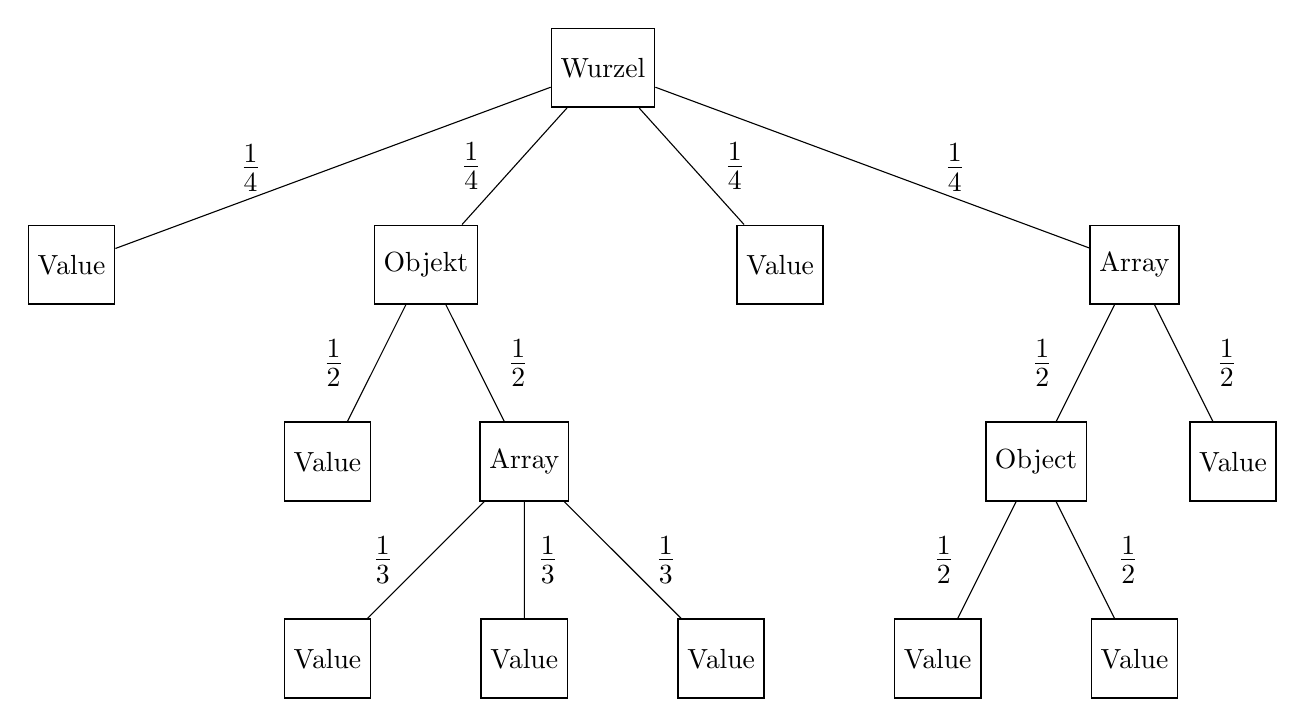
\begin{tikzpicture}[level distance=2.5cm,
  level 1/.style={sibling distance=4.5cm},
  level 2/.style={sibling distance=2.5cm},
  level 3/.style={sibling distance=2.5cm},
  element/.style={draw=black, fill=white, semithick, minimum size=10mm, align=center},
  attribute/.style={ draw=red, fill=white, semithick, minimum size=7mm, align=center},
  textnode/.style={ draw=black, fill=white, semithick, minimum size=7mm, align=center}]
  \node [element](Root){Wurzel}
    child {node [element]{Value}
      edge from parent node[left,font = \Large, outer sep=.80cm]{ \( \frac{1}{4} \)}
    }
    child {node [element]{Objekt}
        child {node [element]{Value} edge from parent node[left,font = \Large, outer sep=.30cm]{ \( \frac{1}{2} \)}}
        child {node [element]{Array}
            child {node [element]{Value} edge from parent node[left,font = \Large, outer sep=.30cm]{ \( \frac{1}{3} \)}}
            child {node [element]{Value} edge from parent node[right,font = \Large, outer sep=0.5mm]{ \( \frac{1}{3} \)}}
            child {node [element]{Value} edge from parent node[right,font = \Large, outer sep=.30cm]{ \( \frac{1}{3} \)}}
        edge from parent node[right,font = \Large, outer sep=.30cm]{ \( \frac{1}{2} \)}}
      edge from parent node[left,font = \Large, outer sep=.30cm]{ \( \frac{1}{4} \)}
    }
    child {node [element]{Value} edge from parent node[right,font = \Large, outer sep=0.3cm]{ \( \frac{1}{4} \)}}
    child {node [element]{Array}
      child {node [element]{Object}
        child {node [element]{Value} edge from parent node[left,font = \Large, outer sep=.30cm]{ \( \frac{1}{2} \)}}
        child {node [element]{Value} edge from parent node[right,font = \Large, outer sep=.30cm]{ \( \frac{1}{2} \)}}
      edge from parent node[left,font = \Large, outer sep=.30cm]{ \( \frac{1}{2} \)}}
      child {node [element]{Value} edge from parent node[right,font = \Large, outer sep=.30cm]{ \( \frac{1}{2} \)}}
      edge from parent node[right,font = \Large, outer sep=.80cm]{ \( \frac{1}{4} \)}
    };
\end{tikzpicture}
    \caption{Beispielbaum für JSON}
    \label{fig:jsonBaum}
\end{figure}

Zunächst werden Knoten über ihre Namen, also ihre Keys gematcht. Sind beide gematchen Knoten vom Typ Value, werden sie nach ihrem Inhalt nach Gleichung (\ref{eq:similarityFunc}) verglichen. Für die Paarung Value- und Arrayknoten wird im Array nach einem Eintrag mit dem Value gesucht. Da das Ziel eine geringe Fehlerquote ist, wird hierbei nur auf exakte Übereinstimmungen geachtet. Andererseits kann hier auch argumentiert werden, dass für eine höchstmögliche Genauigkeit nur Knoten des gleichen Typs verglichen werden sollten. Diese Entscheidung hängt allerdings von der Struktur der Inputdateien ab und ist deshalb nicht eindeutig, weshalb hier auf die Suche im Array gesetzt wird. Value- und Objektknoten werden wiederum nicht miteinander verglichen, da innerhalb des Objekts jedes Element einen eigenen Key hat und es somit keine Möglichkeit gibt, das Value exakt einem Objektelement zuzuordnen. Die einzige Ausnahme wäre, wenn es innerhalb des Objekts ein Element gäbe, welches den gleichen Key hat wie das Elternobjekt. Dieses Element könnte aber auch einen der drei Knotentypen haben weswegen hier auf einen Vergleich verzichtet wird. 

Wenn zwei Arrays miteinander verglichen werden, wird es etwas schwieriger da Arrayelemente weder Keys haben um sie eindeutig zu matchen, noch auf einen bestimmten Elementtyp festgelegt sind. Analog zu den Elementlisten für XML, werden hier zunächst identische Arrayelemente festgestellt und bewertet. Danach folgt die Auswertung der Elementtypen innerhalb der Arrays. Falls Valueknoten innerhalb der Arrays existieren, gelten die gleichen Regeln wie zuvor genannt. Existieren Array-Elemente innerhalb der Arrays, werden diese ebenfalls zunächst durch das Matching ihrer Einträge und dann durch die Fallunterscheidung verglichen. Einträge die nicht gematcht werden konnten, werden in ihrer Reihenfolge verglichen. Zudem werden Arrays und Objekte aufgrund der fehlenden Keys der Arrays nicht miteinander verglichen.

Sollten zwei Objekte innerhalb von Arrays miteinander verglichen oder durch ihre Keys gematcht werden, findet der Vergleich auf Basis der Kindelemente statt. Diese werden über ihre Keys gematcht und je nach Typ mit einer der zuvor genannten Methoden bewertet. 

Die Implementierung basiert im Wesentlichen auf drei Methoden: \emph{compareValues}(), \emph{compareArrays}() und \emph{compareObjects}(). Diese Methoden bekommen als Übergabeparameter die beiden Knoten, die Verglichen werden sollen und liefern ihre Ähnlichkeit zurück. Sie sind so aufgebaut, dass sie sich problemlos gegenseitig aufrufen können, z.\,B. für den Fall dass beim Vergleich von zwei Arrays, zwei Objekteinträge verglichen werden sollen. Zudem funktionieren die beiden Methoden für Arrays und Objekte auch rekursiv, da diese Knotentypen auch Einträge des gleichen Typs beherbergen können.

Das Matching von Arrayeinträgen funktioniert zwar genauso wie das Matching von XML-Elementlisten, die Implementierung weicht aber dadurch ab, dass identische Knoten nicht mehr durch \emph{null} ersetzt werden können, da dies ein gültiger Typ von Valueknoten ist.
Stattdessen wird zu Beginn des Vergleichs ein zufälliger \acrfull{uuid} generiert um einen Wert zu erzeugen, dessen Vorkommen innerhalb einer Datei maximal unwahrscheinlich ist. Um gleiche Arrayeinträge zu finden werden sie mittels der \emph{toString}()-Methode als String dargestellt und über die \emph{equals}()-Methode gematcht. Identische Knoten werden dann im Baum durch einen neuen Arrayknoten ersetzt, welcher lediglich einen Eintrag mit der \acrshort{uuid} beinhaltet. Nach dem Matching werden diese Knoten dann durch die Methode \emph{clearUUIDFields}() entfernt und für den restlichen Vergleich freigegeben. Dafür werden die beiden zu vergleichenden Knoten \emph{fieldValueRef} bzw. \emph{fieldValueComp} mit den veränderten Arrays überschrieben. Dieses Verfahren ist in Quellcode \ref{code:jsonArrayMatching} zu sehen.

\begin{listing}[!t]
\begin{minted}[
frame=lines,
framesep=2mm,
baselinestretch=1.2,
bgcolor=white,
fontsize=\footnotesize,
linenos
]
{java}
        ArrayNode refArray = (ArrayNode) fieldValueRef;
	ArrayNode compArray = (ArrayNode) fieldValueComp;
	for (int i = 0; i < refArray.size(); i++) {
	    String refString = refArray.get(i).toString();
	    for (int j = 0; j < compArray.size(); j++) {
		  String compString = compArray.get(j).toString();
		  if (compString.equals("[\"" + uuid + "\"]")) {
		      continue;
		  }
		  if (refString.equals(compString)) {
		      similarity += currentLevelWeight
				  * calcLevelWeight(fieldValueRef, fieldValueComp);
			  refArray.set(i,objectMapper.createArrayNode()
			 		.add(uuid));
			  compArray.set(j,objectMapper.createArrayNode()
			        .add(uuid));
			  break;
		  }
	    }
	}
	refArray = clearUUIDFields(refArray, uuid);
	compArray = clearUUIDFields(compArray, uuid);
	fieldValueRef = refArray;
	fieldValueComp = compArray;
\end{minted}
\caption{Array-Matching für JSON}
\label{code:jsonArrayMatching}
\end{listing}
%iwas zum matching hier